\chapter[Metodología de Trabajo]{Metodología de Trabajo}
\label{cp:methodology}

\parindent0pt

Para la consecución de los objetivos propuestos en este trabajo final, se ha definido una metodología de trabajo que permite planificar y gestionar las diferentes tareas y recursos del proyecto de manera ordenada. Por ello, en este capítulo se presentan los diferentes pasos que se ejecutaron para llegar a cumplir los objetivos planteados inicialmente. 

Primeramente, se hablará sobre la planificación del trabajo, haciendo hincapié en las actividades necesarias para llevar a cabo el proyecto de forma ordenada y efectiva. Posteriormente, se analizarán distintas metodologías de desarrollo de software, que podrían utilizarse como marco de referencia para la organización de las actividades de desarrollo del prototipo tecnológico, comparando sus características y seleccionando la más adecuada para este trabajo. Finalmente, se describirán las etapas del proceso de desarrollo del prototipo tecnológico, detallando las actividades y resultados esperados en cada una de ellas a partir de la metodología seleccionada.

Definir un plan de trabajo, previo al desarrollo del prototipo tecnológico, es una buena práctica que permite establecer una hoja de ruta concisa que sirve de guía orientativa a lo largo de todo el proceso. Un plan de trabajo es un documento que define los objetivos, actividades y recursos necesarios para llevar a cabo un proyecto de manera efectiva. Para este trabajo en particular, se definió un plan que comprende las actividades necesarias para poder desarrollar un prototipo tecnológico basado en blockchain, orientado a la trazabilidad y valorización del vidrio, con el objetivo de contribuir a la economía circular en la región. Este plan sirve de guía para la ejecución de las actividades y la toma de decisiones a lo largo del proyecto, pero es flexible y puede adaptarse a cambios y nuevas necesidades que puedan surgir durante el desarrollo del trabajo. En la Figura \ref{fig:activities-plan} se ilustran las actividades que conforman el plan de trabajo junto con su duración estimada y secuencialidad. A continuación se detalla el alcance y los objetivos de cada actividad.

\begin{figure}[!htb]
    \centering
    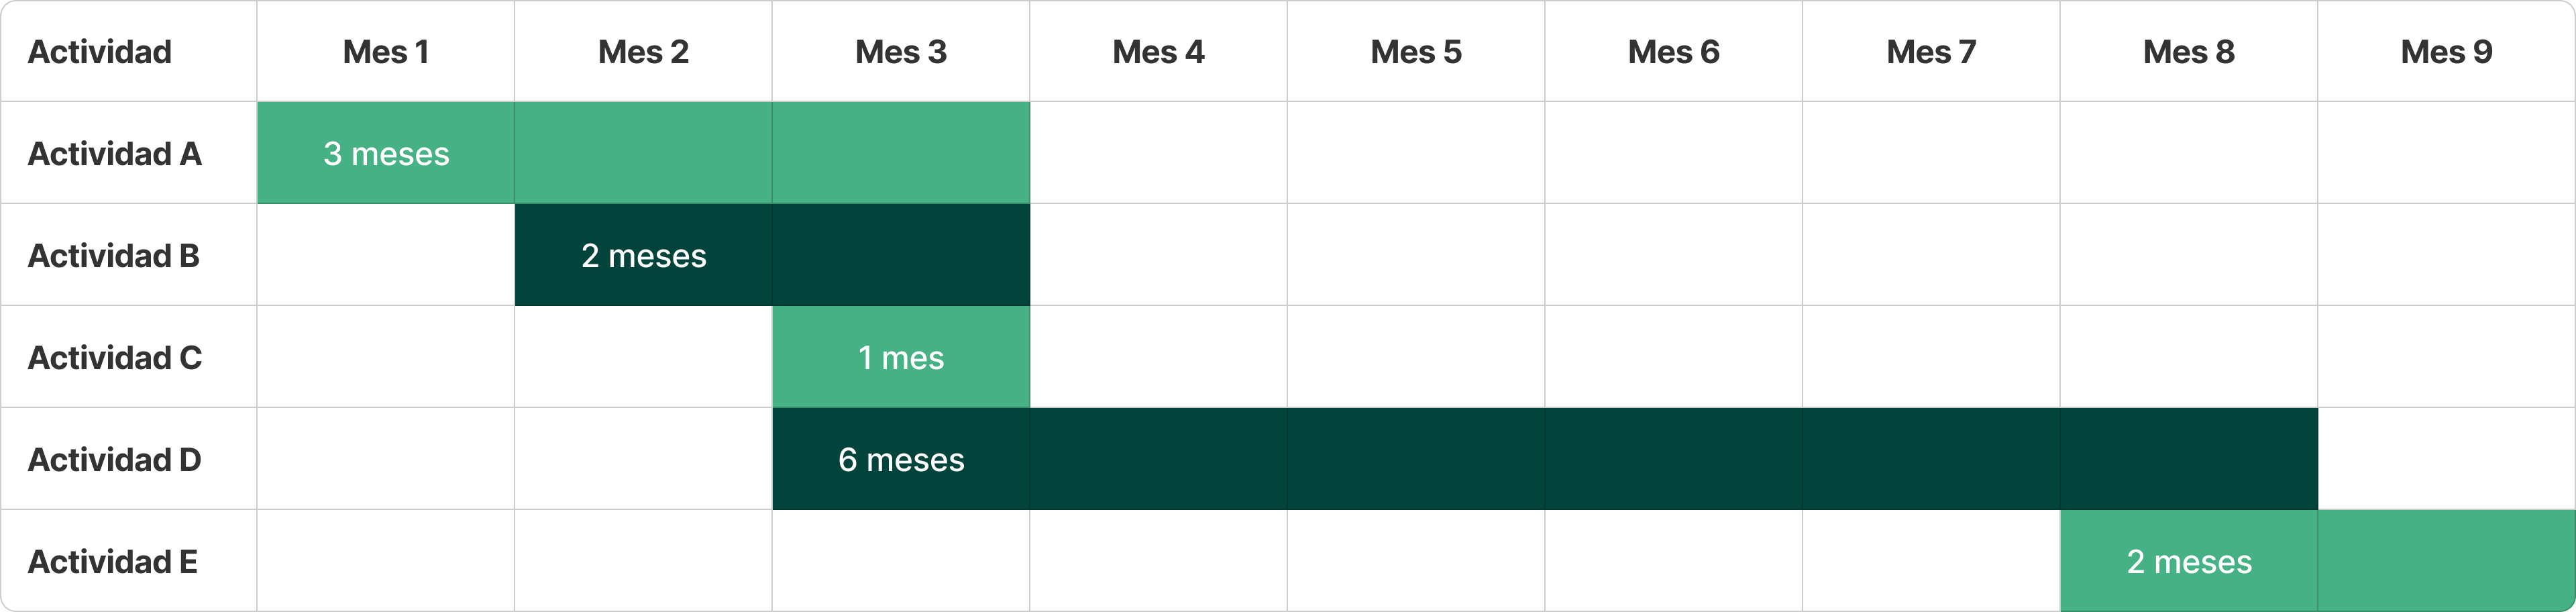
\includegraphics[width=0.8\textwidth]{Figures/activities-plan.png}
    \caption{Organización de las actividades del plan de trabajo}
    \label{fig:activities-plan}
\end{figure}

\begin{itemize}
	\item \textbf{Actividad A}: completar la formación en blockchain y las tecnologías y plataformas relacionadas. Los resultados de esta formación se aplican posteriormente en las etapas de diseño de solución e implementación del prototipo tecnológico (comprendidas en la Actividad D).
	\item \textbf{Actividad B}: realizar un estudio pormenorizado del estado actual del arte en todo lo relacionado con blockchain en el campo del reciclado. En particular, la búsqueda se orienta al reciclado de vidrio. Se analizan trabajos de la literatura, así como aplicaciones blockchain orientadas al reciclaje y la cadena de suministro. Los resultados de este estudio se encuentran documentados en el Capítulo \ref{cp:theoretical-framework}: Marco Teórico y en los Apéndices \ref{cp:verallia-interview}: Entrevista a Verallia y \ref{cp:europe-trip}: Viaje de Investigación.
	\item \textbf{Actividad C}: definir los procesos de desarrollo del prototipo, haciendo hincapié en aplicar los fundamentos de la ingeniería de software y planificar de forma concisa y clara. En la Sección \ref{sec:software-method} se describe la metodología elegida para el proceso de desarrollo del prototipo tecnológico.
	\item \textbf{Actividad D}: desarrollar la aplicación prototipo. Esta actividad comprende las diferentes etapas del proceso de desarrollo de software, desde análisis de requerimientos, diseño, implementación, evaluación, corrección del prototipo y despliegue. Todos estos pasos se deben ejecutar siguiendo la metodología específica elegida para este trabajo durante la Actividad C, teniendo en cuenta las características particulares del modelo de proceso elegido, con el fin de llevar a cabo el objetivo general de este trabajo.
	\item \textbf{Actividad E}: documentar en una memoria el proceso ejecutado y los resultados del trabajo realizado.
\end{itemize}

En la siguiente sección, se hará una comparación de las principales metodologías de desarrollo de software disponibles en la actualidad para seleccionar la más adecuada para este trabajo, teniendo en cuenta las características del proyecto y el equipo de trabajo. 

% TODO: y esto? Lo mato o lo dejo en algún lado?

% \subsection{Delimitación del Alcance}
% El presente trabajo se centra en la tecnología blockchain como eje principal debido a su naturaleza disruptiva y su potencial para transformar la trazabilidad y la gestión de datos. La elección de la aplicación orientada a la economía circular se justifica por la relevancia actual de este área de impacto y la necesidad de soluciones sostenibles. Particularmente, el dominio se delimita al vidrio, siguiendo la recomendación de diversas investigaciones que sugieren que la especialización en un material particular permite obtener mejores resultados en usabilidad y tasas de reciclaje \cite{pending}. Esto se debe a la posibilidad de diseñar sistemas a medida de los procesos productivos y de reciclaje del material elegido. El vidrio en particular es seleccionado como material reciclable para desarrollar este trabajo por sus características de alta reciclabilidad y su significativo impacto regional en Mendoza (provincia vitivinícola) cuya principal industria productiva, el vino, depende en gran medida de los envases de vidrio. La localización en Mendoza se debe a que este trabajo se desarrolla en la Universidad Nacional de Cuyo (UNCUYO), con sede principal en esta provincia.

\section{Metodología de Desarrollo}
\label{sec:software-method}

En la actualidad, existen diversas metodologías de desarrollo de software que permiten planificar y ordenar el proceso de desarrollo de software para lograr obtener resultados que cumplan con los objetivos del proyecto haciendo un uso eficiente de los recursos disponibles. Cada metodología tiene sus propias características, ventajas y desventajas, y la elección de una metodología apropiada depende de las necesidades específicas del proyecto, el equipo de trabajo y los objetivos a alcanzar.

El objetivo principal de esta sección es realizar un análisis detallado de las principales metodologías de desarrollo de software conocidas, evaluando sus características y su aplicabilidad en función de los requerimientos y condiciones particulares del trabajo de tesis. Para ello, se realiza un análisis de las principales metodologías de desarrollo de software vigentes en la industria del software, cada una con enfoques y principios diferentes, pero con un mismo fin: facilitar el desarrollo de un software funcional que cumpla con los objetivos planteados. Como parte del análisis, se compara cada metodología en función de varios criterios relevantes para este trabajo, como la definición de requerimientos, la planificación de actividades, el alcance del prototipo, el tamaño del equipo, la frecuencia de entrega de resultados y la flexibilidad frente a cambios de requerimientos.

Las metodologías de desarrollo de software pueden clasificarse en dos grandes categorías: los modelos prescriptivos o tradicionales, que ofrecen una estructura y un orden definidos para maximizar la previsibilidad y la eficiencia en entornos estables, y los modelos evolutivos o ágiles, que se adaptan mejor a las realidades dinámicas del desarrollo de software moderno al permitir la iteración continua y la flexibilidad frente a los cambios. A continuación, se describe cada una de las principales metodologías consideradas para este trabajo.

Dentro de los enfoques tradicionales, el modelo en cascada es el más conocido, un modelo secuencial y lineal donde las fases del proyecto deben completarse en un orden estricto, desde la especificación de requerimientos hasta el despliegue y mantenimiento. Cada una de las etapas del proceso debe ser completada satisfactoriamente antes de avanzar a la siguiente. Si bien su rigidez lo hace ideal para proyectos con requisitos estables, esta misma característica le impide adaptarse a cambios, lo que puede llevar a costos adicionales y retrasos si surgen nuevas necesidades o se descubren errores durante el desarrollo. Por esta razón, el modelo en cascada es ideal para proyectos donde los requerimientos son bien conocidos y estables desde el inicio.

\begin{figure}[h]
    \centering
    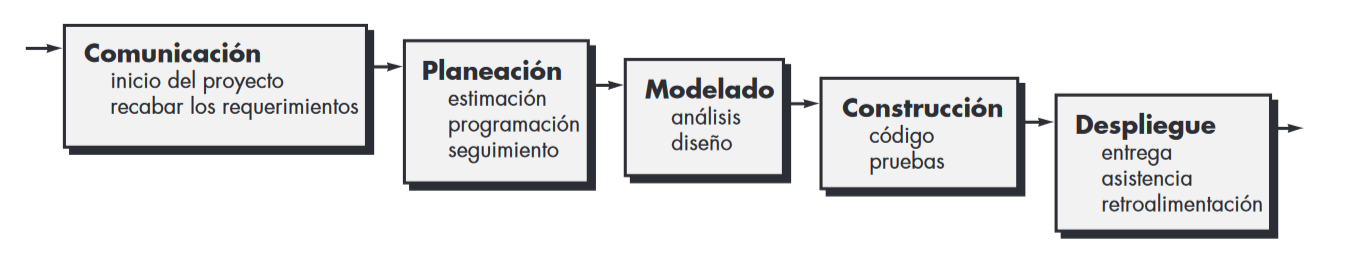
\includegraphics[width=\linewidth]{Figures/model-waterfall.png}
    \caption{Modelo en cascada. Fuente: \cite{pressman2010ingenieria}}
\end{figure}

Otra opción considerada dentro de los enfoques tradicionales es el modelo en V, una extensión del modelo en cascada que empareja cada fase de desarrollo con una fase de prueba correspondiente. Esta estructura en forma de ``V`` busca una verificación sistemática en cada etapa, con el fin de detectar y corregir errores de forma temprana y minimizar riesgos al final del proyecto. A medida que el proyecto avanza hacia abajo en la primera mitad de la V, los requisitos y componentes del sistema son detallados cada vez más. Una vez completada la codificación, el proceso asciende por el lado derecho de la V, donde cada etapa de desarrollo anterior es validada a través de pruebas específicas. Este modelo es apropiado para proyectos que requieren altos estándares de calidad y donde los errores tempranos podrían tener consecuencias costosas o críticas. Aunque este modelo comparte algunas limitaciones con el modelo en cascada, como la dificultad para adaptarse a cambios significativos una vez que el proyecto está en curso, su estructura permite una mejor gestión del riesgo y calidad mediante la validación constante de cada etapa del desarrollo.

\begin{figure}[!htb]
	\centering
	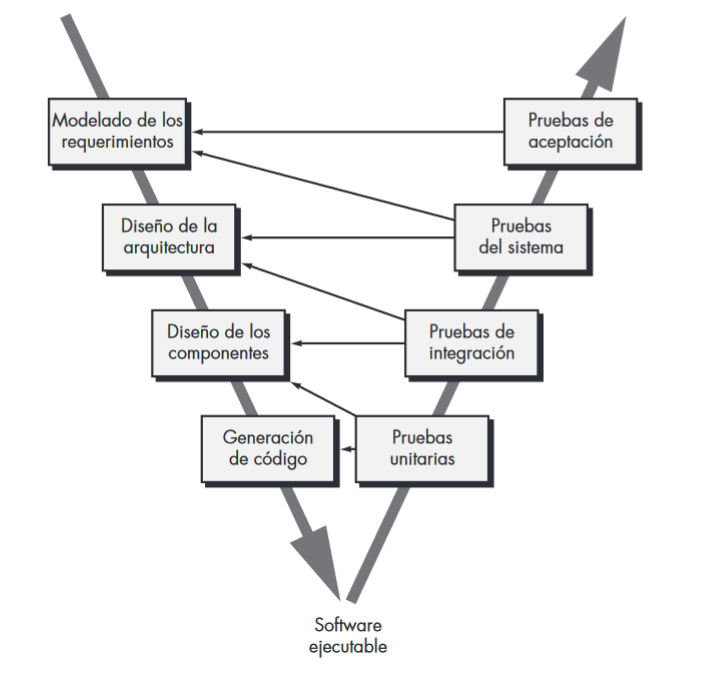
\includegraphics[width=0.6\textwidth]{Figures/model-v.png}
	\caption{Modelo en V. Fuente: \cite{pressman2010ingenieria}}
\end{figure}

Dentro del conjunto de modelos evolutivos, el modelo espiral es un enfoque destacado por combinar la iteración flexible de los prototipos con la rigurosidad sistemática del modelo en cascada \cite{pressman2010ingenieria}. Se distingue por su enfoque cíclico, diseñado para permitir el crecimiento incremental de un sistema mientras se gestionan y reducen los riesgos. La flexibilidad de esta metodología reside en su capacidad para adaptarse continuamente a las necesidades cambiantes del proyecto a través de iteraciones sucesivas. En cada ciclo de la espiral, el proceso contempla la planificación, la identificación de riesgos, el desarrollo y la evaluación de un prototipo o una sección del software, para luego planificar la siguiente iteración. Este enfoque iterativo permite a los desarrolladores y actores involucrados entender mejor los riesgos y reaccionar ante ellos en cada etapa del proyecto. El modelo espiral es particularmente útil en entornos dinámicos y en constante cambio, aunque su principal desafío radica en la necesidad de una evaluación continua y experta de los riesgos, lo que puede aumentar la complejidad de la gestión del proyecto.

\begin{figure}[!htb]
    \centering
    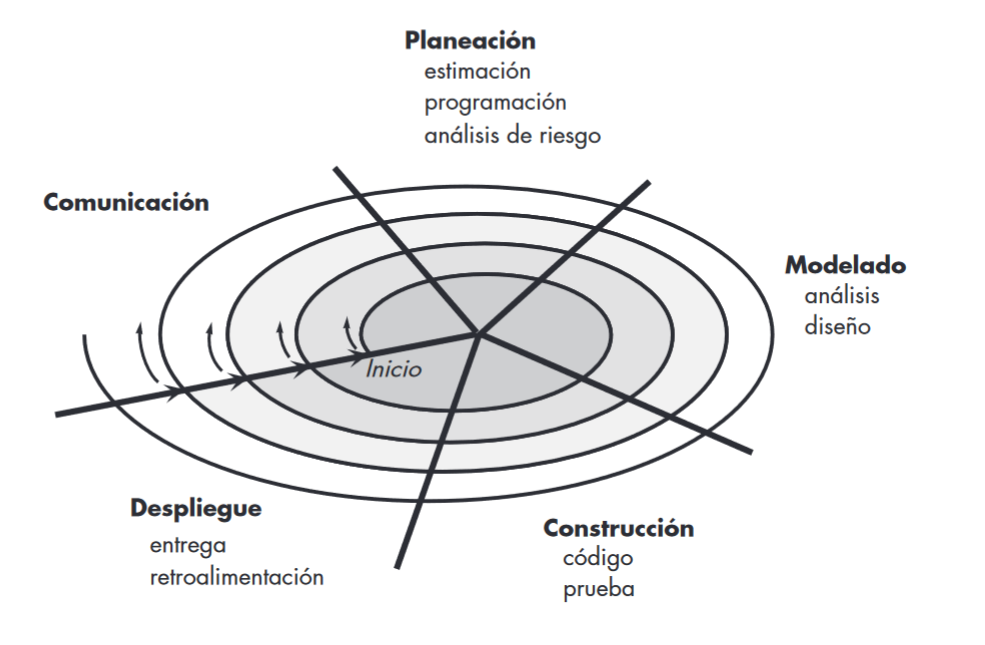
\includegraphics[width=0.6\textwidth]{Figures/model-spiral.png}
    \caption{Modelo espiral. Fuente: \cite{pressman2010ingenieria}}
\end{figure}

Por otro lado, Scrum es una metodología ágil de desarrollo de software que se alinea con los principios del Manifiesto Ágil, promoviendo la flexibilidad, la colaboración continua y la adaptabilidad a los cambios \cite{pressman2010ingenieria}. Este modelo estructura el desarrollo en ciclos cortos y repetitivos denominados \textit{sprints}, típicamente de dos semanas. Al comenzar cada sprint, se seleccionan las tareas que se abordarán de la lista de pendientes del proyecto. Durante un sprint, no se permiten cambios en los requisitos, lo que proporciona estabilidad mientras el equipo aborda las tareas seleccionadas. El proceso incluye reuniones diarias breves, que ayudan a identificar y resolver problemas rápidamente y fomentan la autogestión del equipo. Al final de cada sprint, se presenta una demostración del incremento de software desarrollado, lo que facilita la retroalimentación hacia el equipo para influir en los siguientes incrementos. Scrum es particularmente efectivo en entornos donde la incertidumbre es alta, ya que permite la iteración continua y la evaluación constante de riesgos, haciendo que el proyecto se adapte a las expectativas de las distintas partes interesadas y a las circunstancias cambiantes. A su vez, su enfoque en la colaboración y la comunicación constante, hace que esta metodología sea apropiada para equipos medianos y grandes, donde la coordinación es importante y las reuniones diarias no representan una sobrecarga, sino una oportunidad para alinear esfuerzos y resolver impedimentos.

\begin{figure}[!htb]
    \centering
    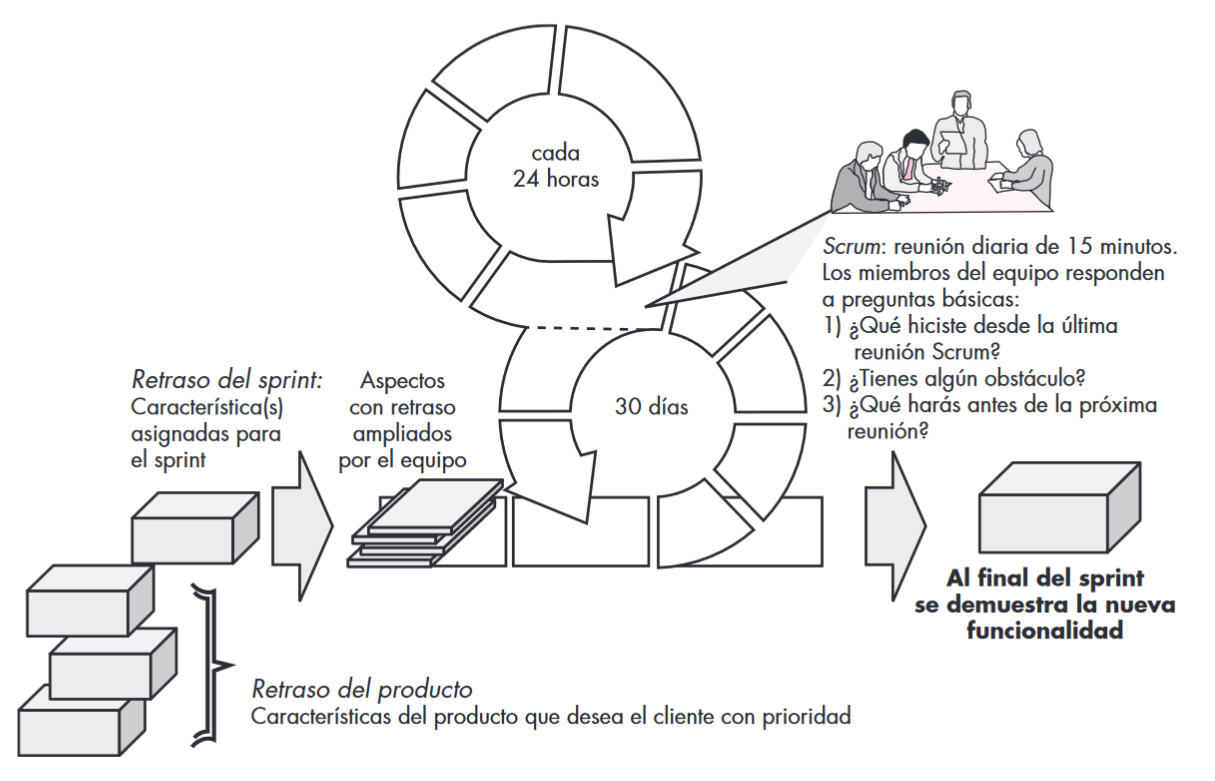
\includegraphics[width=0.6\textwidth]{Figures/model-scrum.png}
    \caption{Metodología Scrum. Fuente: \cite{pressman2010ingenieria}}
\end{figure}

Finalmente, el método Kanban es un enfoque visual para la gestión del flujo de trabajo, cuyo objetivo principal es optimizar la eficiencia al prevenir la sobrecarga de tareas y eliminar cuellos de botella \cite{alaidaros2021kanban}. Se centra en un sistema dinámico, donde el trabajo solo se inicia cuando hay capacidad disponible, lo que se traduce en una mayor adaptabilidad y una respuesta más rápida a los cambios en las prioridades del proyecto. Este método propone implementar un tablero visual dividido en columnas que representan las diferentes etapas del proceso de desarrollo, por donde se mueven las tareas o tarjetas. Los principios de este modelo incluyen limitar el trabajo en curso, visualizar el flujo de tareas y medir su progreso para reconocer oportunidades de mejora. Kanban es una metodología de implementación ligera que se adapta bien a la situación actual de cualquier organización, es compatible con otras metodologías de trabajo y su implementación no requiere cambios estructurales. Sin embargo, su eficacia depende de una disciplina rigurosa y una comunicación constante para asegurar que el flujo visualizado en el tablero refleje la realidad actual del estado del proyecto.

\begin{figure}[!htb]
    \centering
    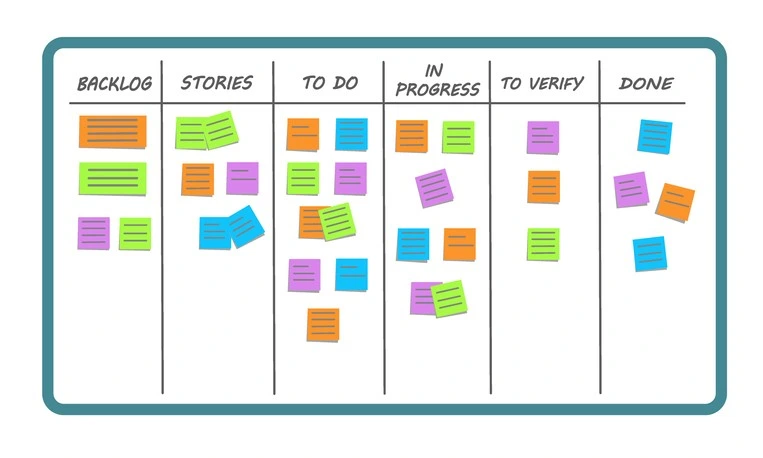
\includegraphics[width=0.6\textwidth]{Figures/model-kanban.png}
    \caption{Tablero Kanban de ejemplo.}
\end{figure}

Para el desarrollo del presente trabajo, se busca seleccionar una metodología que se adapte a las características del proyecto. Por lo tanto, el proceso de selección de metodología comienza prescindiendo aquellos enfoques que no se ajustan a las necesidades y características del proyecto. En primer lugar, se desestima el uso de la metodología Scrum debido a que requiere una participación activa y constante de un cliente para guiar los sprints, un rol que no es factible en el contexto de un proyecto académico individual. A su vez, las reuniones recurrentes de esta metodología pierden sentido en un equipo unipersonal, donde la comunicación constante y la coordinación del equipo no son necesarias. Por otro lado, el modelo Espiral no se considera apropiado para este trabajo debido a su alta complejidad para el alcance del prototipo. Este modelo se centra en la gestión de riesgos y la adaptación continua a los cambios. Sin embargo, dado que los requisitos de este trabajo están claramente definidos y la investigación y el análisis previos han minimizado la incertidumbre, la complejidad y el tiempo adicional que el modelo Espiral implicaría no se justifican para este proyecto.

Luego de prescindir los enfoques mencionados, la selección de metodología se centró en los modelos restantes, principalmente en Modelo en V y Kanban. Ambos modelos se consideran apropiados para el desarrollo de este trabajo y su implementación es mutuamente compatible. El Modelo en V aporta un enfoque estructurado para la planificación y documentación del proyecto, mientras que Kanban proporciona flexibilidad para la gestión de tareas y el seguimiento del flujo de trabajo diario en un entorno unipersonal. La naturaleza visual de Kanban facilita el seguimiento del progreso y permite una adaptación ágil a los cambios menores que puedan surgir en el día a día, sin comprometer la estructura general del proyecto. A su vez, el modelo en V resulta más apropiado respecto al modelo en cascada debido a su foco en la verificación y validación de los resultados de cada etapa del proceso de desarrollo. Este enfoque de validación continua resulta especialmente valioso para este trabajo, ya que la inmutabilidad de los contratos inteligentes desplegados en la blockchain, hace que la detección temprana de errores sea crítica para garantizar la calidad y la fiabilidad del prototipo final. 

Finalmente, para este trabajo se elige aplicar una combinación de modelos, utilizando el modelo en V para la planificación y estructura general del proceso de desarrollo, y Kanban para la gestión de tareas diarias y el seguimiento del progreso del proyecto. Esta combinación busca mantener un enfoque sistemático y estructurado, al mismo tiempo que se aprovecha la flexibilidad operativa que Kanban ofrece para adaptarse a los cambios menores que puedan surgir durante el desarrollo del prototipo. El siguiente apartado abordará en detalle cada etapa del proceso de desarrollo en el contexto del modelo en V, desde el modelado de requerimientos hasta las pruebas, para llevar a cabo el desarrollo del prototipo tecnológico.

\subsection{Etapas del Proceso de Desarrollo}

Una vez seleccionada la metodología de desarrollo, se procede a la ejecución de las fases de construcción y validación del prototipo. Utilizando el Modelo en V como marco de referencia, el desarrollo del sistema se concibe como un proceso estructurado que se divide en dos grandes fases: la fase descendente, que se enfoca en la definición, el diseño y la implementación, y la fase ascendente, que se centra en la verificación y las pruebas. A continuación, se detallan las actividades y los resultados esperados de cada una de las etapas del proceso de desarrollo, siguiendo el modelo en V, aplicado al prototipo de trazabilidad del vidrio basado en blockchain. En la Figura \ref{fig:methodology-v-grouped} se muestran las etapas del proceso de desarrollo en V agrupadas en bloques temáticos, con el fin de ilustrar de manera más clara las interacciones y dependencias entre las diferentes fases de desarrollo de este trabajo.

\begin{figure}[!htb]
	\centering
	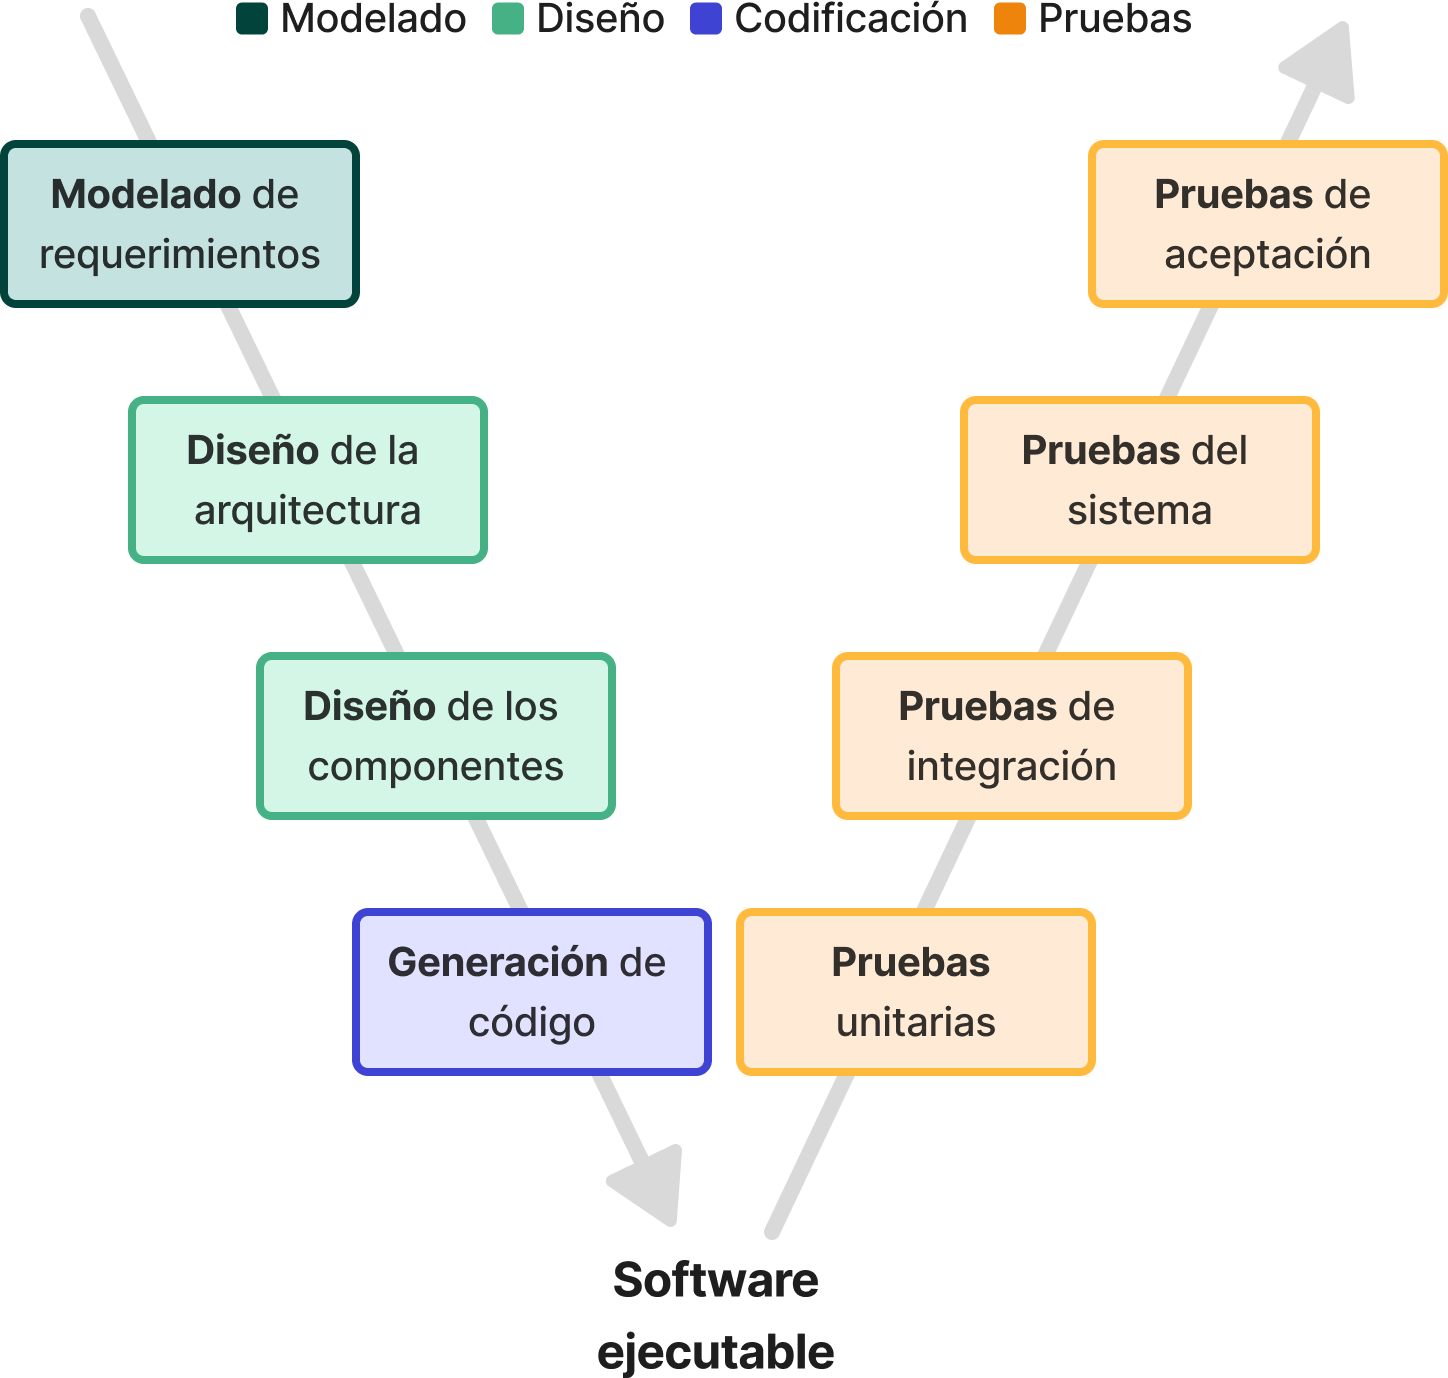
\includegraphics[width=0.6\textwidth]{Figures/model-v-grouped.png}
	\caption{Modelo en V agrupado por etapas. Fuente: \cite{pressman2010ingenieria}}
    \label{fig:methodology-v-grouped}
\end{figure}


\textbf{Modelado de requerimientos:}
Es la primera fase del proceso, comprende la identificación y documentación detallada de los requisitos funcionales y no funcionales del prototipo.
Los hallazgos se nutren directamente de la investigación realizada como parte de la Actividad B, comprendiendo la revisión del estado del arte en blockchain, gestión de residuos y trazabilidad, así como las entrevistas y las observaciones de programas de reciclaje existentes.
El objetivo en esta etapa es comprender las necesidades específicas del sistema de trazabilidad del vidrio para definir un conjunto exhaustivo de requerimientos que aseguren que el prototipo aborde los desafíos identificados en la cadena de producción de envases de vidrio en la región.
El resultado de esta fase es un documento de requisitos funcionales y no funcionales que sirve como guía para las siguientes etapas del desarrollo.
La ejecución y resultados de esta fase se detallan en el Capítulo \ref{cp:modelling}.

\textbf{Diseño:}
El diseño del sistema se divide en dos etapas: diseño de arquitectura y diseño de componentes.
En la primera etapa, se define la arquitectura general del sistema, incluyendo la selección de tecnologías y plataformas a utilizar, así como la estructura de los módulos principales y la división de responsabilidades entre ellos.
En la segunda etapa, se realiza el diseño detallado de cada componente de los módulos del sistema, especificando las interfaces, protocolos de comunicación y estructuras de datos a utilizar.
El diseño en etapas y previo a la implementación tiene el objetivo de garantizar que el sistema sea escalable, mantenible y cumpla con los requisitos definidos en la fase anterior.
El resultado es un conjunto de documentos de diseño que guían la implementación del prototipo.
Los detalles de estas dos fases de diseño se presentan en el Capítulo \ref{cp:design}.

\textbf{Generación de código:}
Durante la fase de generación de código o implementación, se lleva a cabo la codificación del prototipo, cada módulo y sus componentes en las tecnologías elegidas y especificaciones detalladas durante la etapa de diseño.
Esta etapa es gestionada con el apoyo de Kanban para la organización y seguimiento de las micro-tareas para mantener un flujo de trabajo ágil y adaptable a los cambios menores que puedan surgir durante el desarrollo.
El resultado de esta fase es un prototipo funcional que implementa los requisitos y diseños definidos previamente.
En simultáneo con la generación de código se realiza la primera etapa de validación, que consiste en pruebas unitarias de cada componente desarrollado.
Estas pruebas aseguran que cada componente funcione correctamente de forma aislada y cumpla con los requisitos funcionales especificados.
Al finalizar esta etapa, el software ejecutable está listo para ser desplegado en un entorno de pruebas.
Los detalles de la implementación y las pruebas unitarias se describen en el Capítulo \ref{cp:implementation}.

\textbf{Pruebas:}
El proceso de pruebas se lleva a cabo en múltiples etapas.
Después de las pruebas unitarias, se realizan pruebas de integración automatizadas para verificar que los diferentes módulos del sistema interactúan correctamente entre sí a través de sus interfaces.
Estas pruebas aseguran que los datos fluyan adecuadamente dentro del sistema.
Posteriormente, se llevan a cabo pruebas de sistema para evaluar el comportamiento del prototipo en su conjunto para validar que el sistema cumple con los requisitos funcionales y no funcionales definidos.
Las pruebas de sistema incluyen pruebas manuales para validar consistencia de datos en el sistema y corroborar que el prototipo cumple con los requerimientos funcionales, junto con pruebas automatizadas mediante código, que permiten verificar los requerimientos no funcionales como rendimiento y seguridad bajo condiciones simuladas.
Finalmente, se realizan pruebas de aceptación con un conjunto de usuarios voluntarios para validar que el prototipo cumple con los criterios de aceptación establecidos en la fase de modelado de requerimientos.
Los detalles de las pruebas realizadas en estas etapas de pruebas se presentan en el Capítulo \ref{cp:testing}.

Para asegurar una gestión eficiente a lo largo de todas las fases del proceso de desarrollo, se implementan herramientas y prácticas de control de proyectos. La documentación del proceso es continua, registrando las decisiones de diseño, los problemas encontrados y las soluciones aplicadas, lo que sirve como base para la elaboración del informe final. Para el control de versiones del código fuente, se utiliza Git, una herramienta que permite un seguimiento detallado, seguro y ordenado de los cambios en el código. Adicionalmente, se emplea la herramienta Jira, un software de gestión de proyectos para el seguimiento de tareas y la evolución general del desarrollo mediante un tablero Kanban, facilitando la planificación, el monitoreo del progreso y la gestión de tareas pendientes. Esta combinación de herramientas y metodologías permite mantener un flujo de trabajo organizado, transparente y eficiente, alineado con las necesidades específicas del proyecto.

En los próximos capítulos se detallará el proceso de ejecución llevado a cabo en cada una de las etapas descritas, incluyendo los resultados obtenidos en cada una.
En el Capítulo \ref{cp:modelling} se describirá el proceso de modelado de requerimientos, donde se explica cómo se obtuvieron los requerimientos funcionales y no funcionales, su priorización y la planificación del desarrollo.
En el Capítulo \ref{cp:design} se abordará el diseño del sistema, incluyendo la elección de tecnologías, diseño de arquitectura de software, modelado de la interfaz de usuario y definición de los módulos principales del prototipo.
Seguidamente, en el Capítulo \ref{cp:implementation} se detallará la implementación de cada módulo del sistema, integración de los módulos, pruebas unitarias realizadas y despliegue del prototipo en un entorno de pruebas similar a un entorno productivo.
En el Capítulo \ref{cp:testing} se describirán las pruebas realizadas, tanto las pruebas de integración automatizadas como las pruebas de sistema manuales y las pruebas con usuarios.
Finalmente, en el Capítulo \ref{cp:conclusions} se presentarán las conclusiones del trabajo, resultados obtenidos, reflexiones sobre el proceso de desarrollo y oportunidades de mejora de este trabajo con recomendaciones para futuros trabajos relacionados con la trazabilidad y valorización del vidrio mediante tecnologías emergentes como blockchain.
